%%
%%  Department of Electrical, Electronic and Computer Engineering.
%%  EPR400/2 Project Proposal - Section 3.
%%  Copyright (C) 2011-2017 University of Pretoria.
%%

\section*{3. Functional analysis}
\addcontentsline{toc}{subsection}{3. Functional analysis}

The functional analysis of the system can be shown best in a flow diagram. This can be seen in Figure \ref{fig:Func} below.

\begin{figure}[H]
\centering
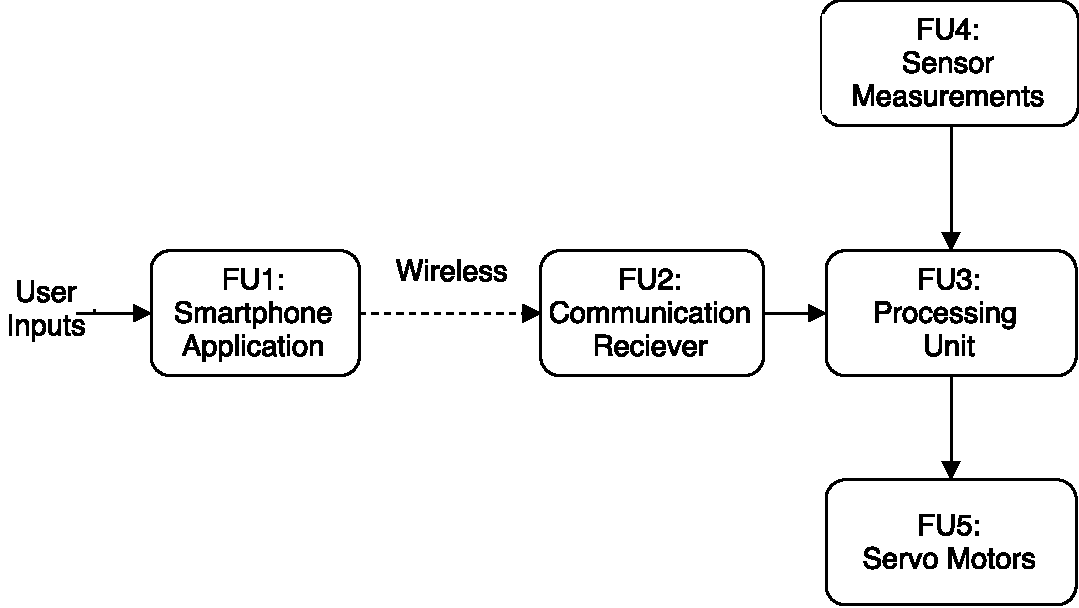
\includegraphics[scale=0.8]{Proposal/FunctionalDiagram.pdf}
\caption{Functional block diagram of the product.}
\label{fig:Func}
\end{figure}

In Figure \ref{fig:Func} above, the process is shown to begin with the input from the user into a smartphone application. This consists of a user interface on the screen of the smartphone that the user can interact with. The user interface will allow the user to make the robot translate as well as rotate. This information is sent to the microcontroller on the robot via wireless technology.
The robot analyses this combination of translation and rotation commands and breaks it into a separate vector for each of the legs. The final position of each leg as well as the route to each individual leg destination is computed next. This makes use of a process called inverse kinematics. The manoeuvres requested by the user can be realized through a series of movements with servo motors installed on the joints of the robot legs. In order to make a limb move, the exact required angle of each joint is calculated and communicated to the servo. This process is repeated continuously to make the robot react to the varying inputs of the user.

\newpage

%% End of File.

